\section{Methodology}

\subsection{Methodological approach}

\paragraph{}
The aim of this research is to address a theoretical research problem; summarization of large scale streaming graphs. Since graph summarization techniques have to be evaluated and benchmarked against each other, quantitative methods best suit this research. Internal validity of the research can be ensured as the causal relationship that will be tested is trustworthy and not influenced by any other factors. Since this is algorithmic research, the simulated experimentation environment can be almost similar to a real-world scenario.

\subsection{Research assumptions}

\begin{enumerate}
    \item Graph stream is simulated by reading a database of stored edges. It is assumed that no interruption occurs during the streaming process, thus creating an idle streaming environment.
    \item The streaming is made to happen at a uniform rate as the information about the rate of streaming is not included with the used datasets.
\end{enumerate}

\subsection{Data collection methods}

\paragraph{}
For this research, mostly large real-world graphs will be used. These datasets can belong to different application domains such as social networks, network packet routes or even a citation network. When selecting the datasets an extra effort will be taken to ensure that they are as different from each other as possible.

\paragraph{}
The experiments will consist of testing the graph summarization algorithms with the collected data and measuring various aspects such as memory consumption, the average error against each other.

\subsection{Data analysis procedures}

\paragraph{}
Quantitative analysis methods will be used when analyzing the results obtained by running different sketching algorithms on obtained datasets. This research belongs to the experimental type as indicated in \autoref{fig:methodology}.

\begin{figure}[H]
    \centering 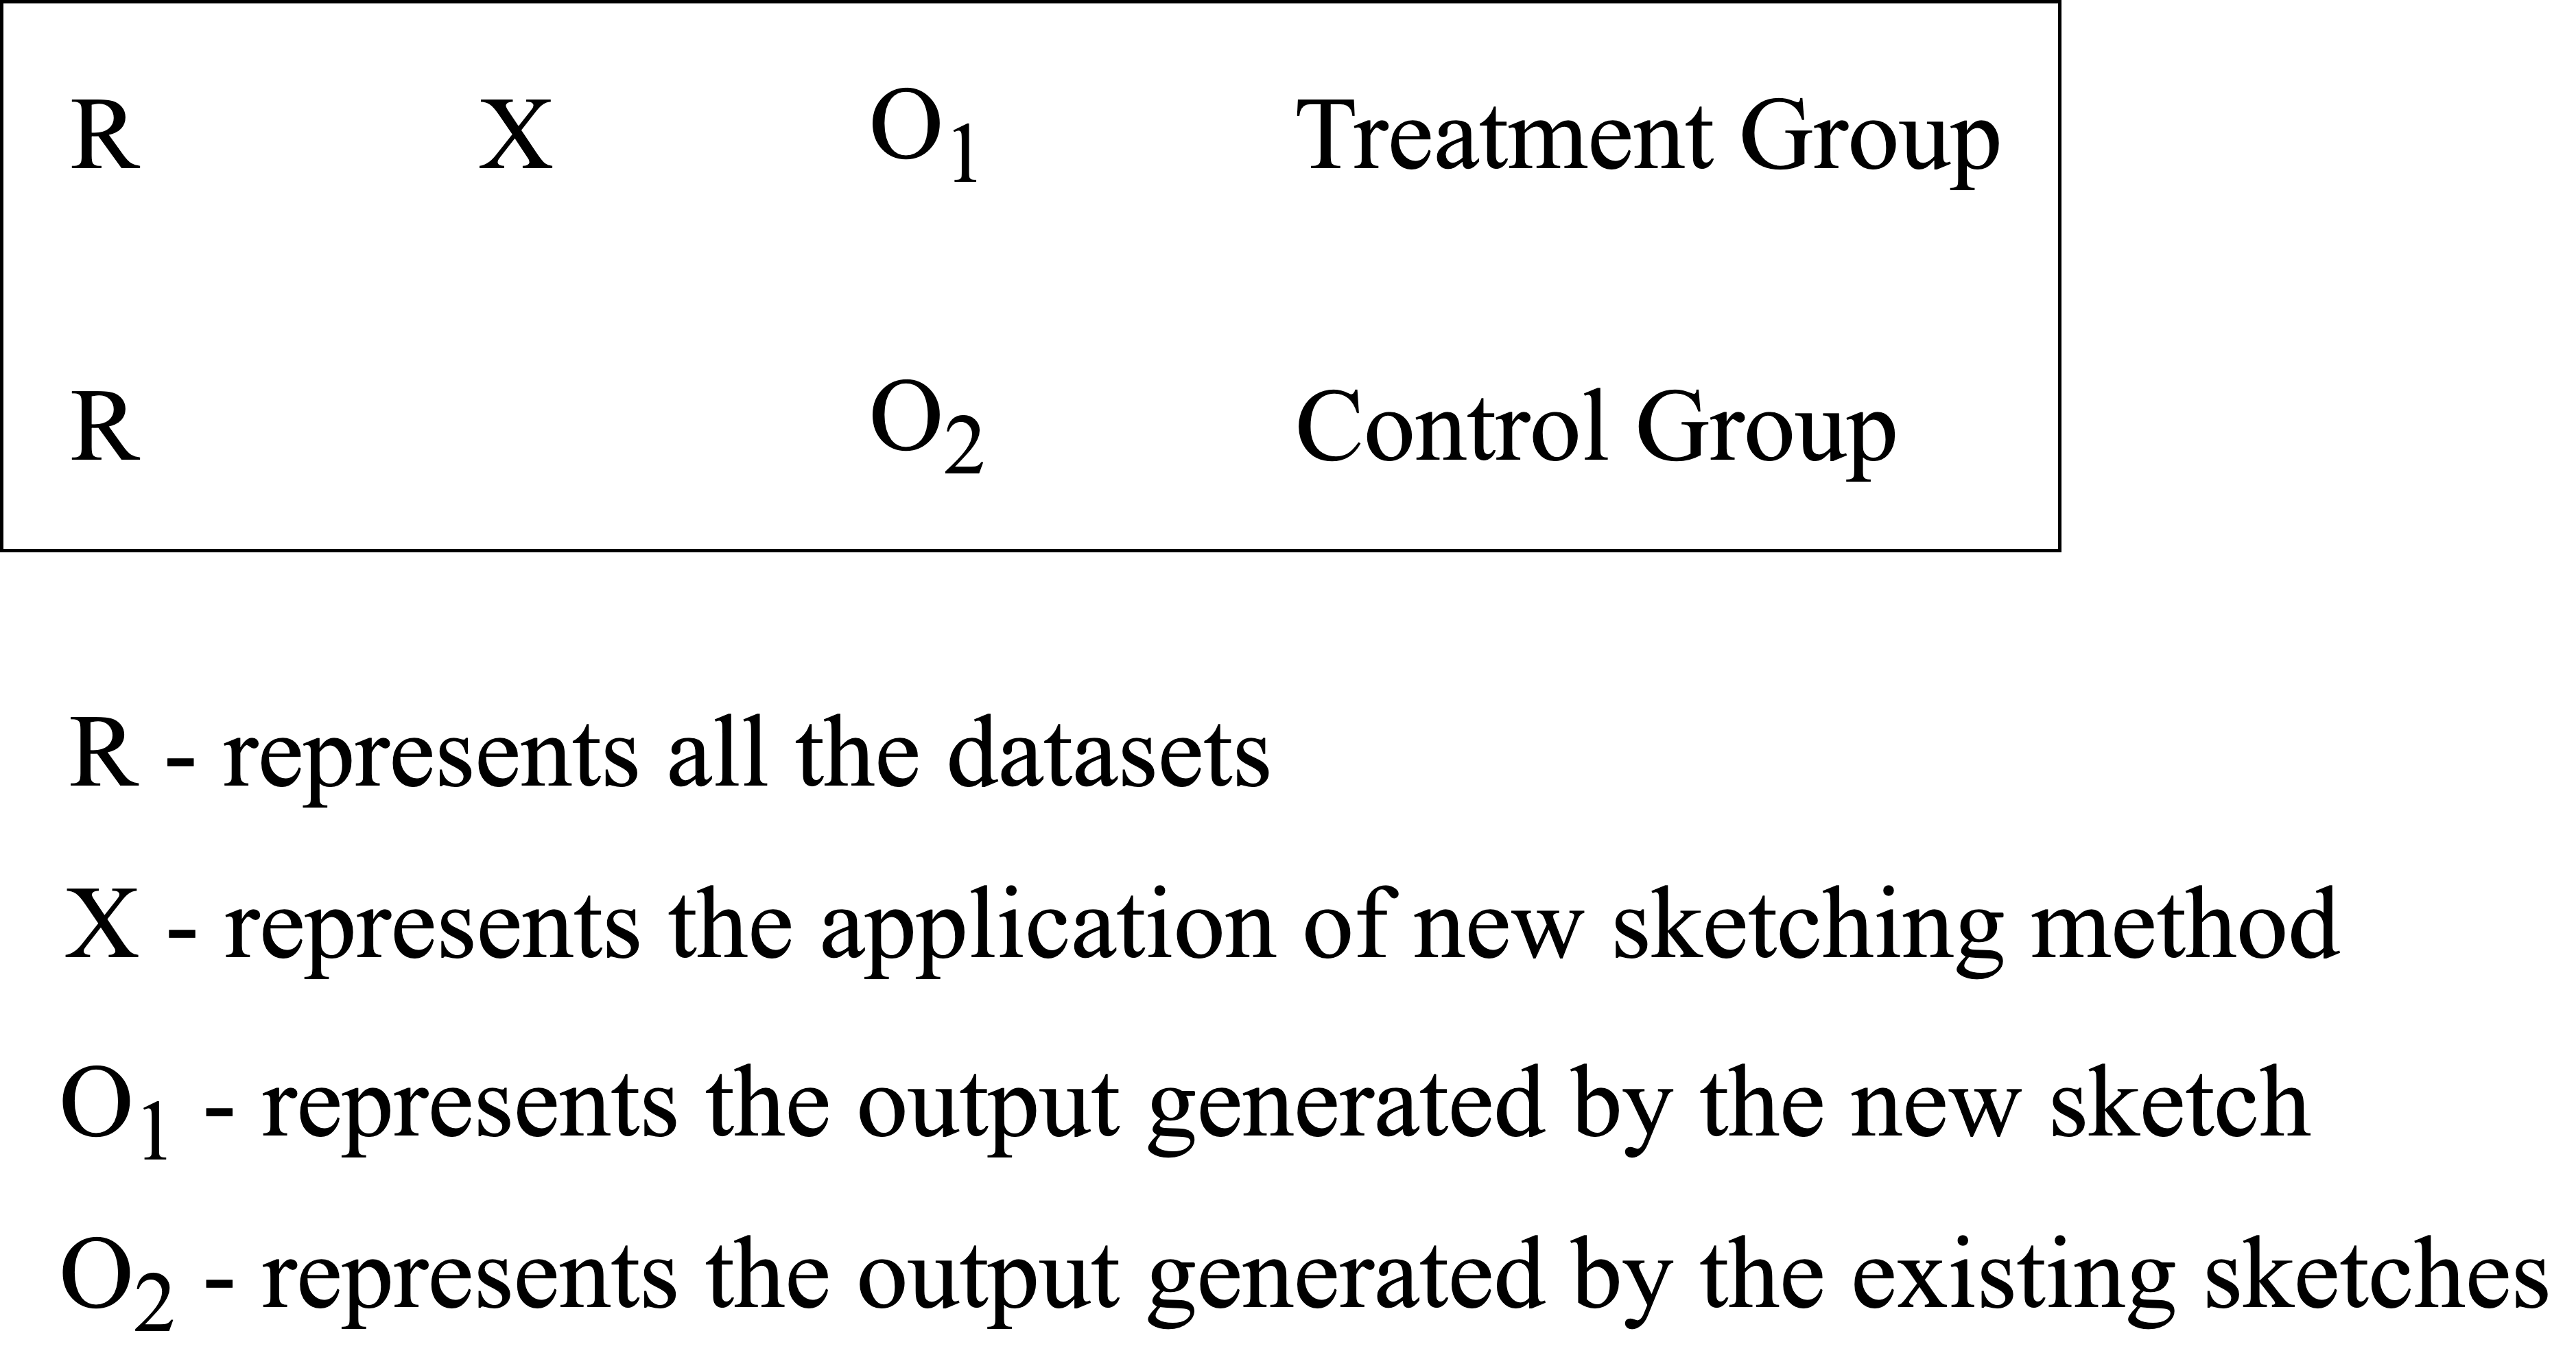
\includegraphics[width=0.7\textwidth]{methodology}
    \caption{Research methodology}
    \label{fig:methodology}
\end{figure}